\section{Level 1 Decompositions}
\label{sec:level-1}

\npar In the first level, the whole system, ReMeS is decomposed. 

\subsection{ReMeS (Whole System)}
\label{dec:whole-system}

\npar In the first step of the ADD process, the whole system is decomposed in
two subsystems ``Remote Module Subsystem'' and ``Portal''. The decomposition is
shown in figure \ref{fig:dec/level-1}.

\begin{figure}[H]
	\begin{centering}
		% TODO
		%\includegraphics[width=0.6\textwidth]{figs/decomposition/whole-system/decomposition.pdf}
		\caption{The level 1 decomposition of the ReMeS system}
		\label{fig:dec/level-1}
	\end{centering}
\end{figure}

\subsubsection{Architectural Drivers}
\label{drivers:whole-system}

\npar For the first decomposition, two high priority quality attribute scenarios
and their associated use cases are taken into account. 

\begin{itemize}
 	\item Av1 (High): Measurement database Failure
 	\begin{itemize}
 		\item UC8 (High): Send measurement
 		\item UC13 (High): Send alarm 
 	\end{itemize}
  	\item P1 (High): Timely closure of valves
  	\begin{itemize}
  		\item UC13 (High): Send alarm 
		\item UC11 (Medium): Operate actuator remotely 
  	\end{itemize}
\end{itemize}

\npar The considered use cases includes the use cases listed below. 

\begin{itemize}
	\item UC7 (High): Send trame to remote device
	\item UC9 (High): Notify customer
	\item UC10 (Medium): Detect anomaly
\end{itemize}

\npar Based on the architectural drivers, the remote module subsystem has to
provide functionality for remote module communication (receiving and sending
trames), trame storage, trame processing and customer communication. 

\npar In order to obtain a better understanding of the relationships between
these functionalities, a small domain model is drafted. Figure
\ref{fig:dec/whole-system/draft} This model can then be refined later on
in this level of decomposition.

\begin{figure}[H]
	\begin{centering}
		% TODO
		%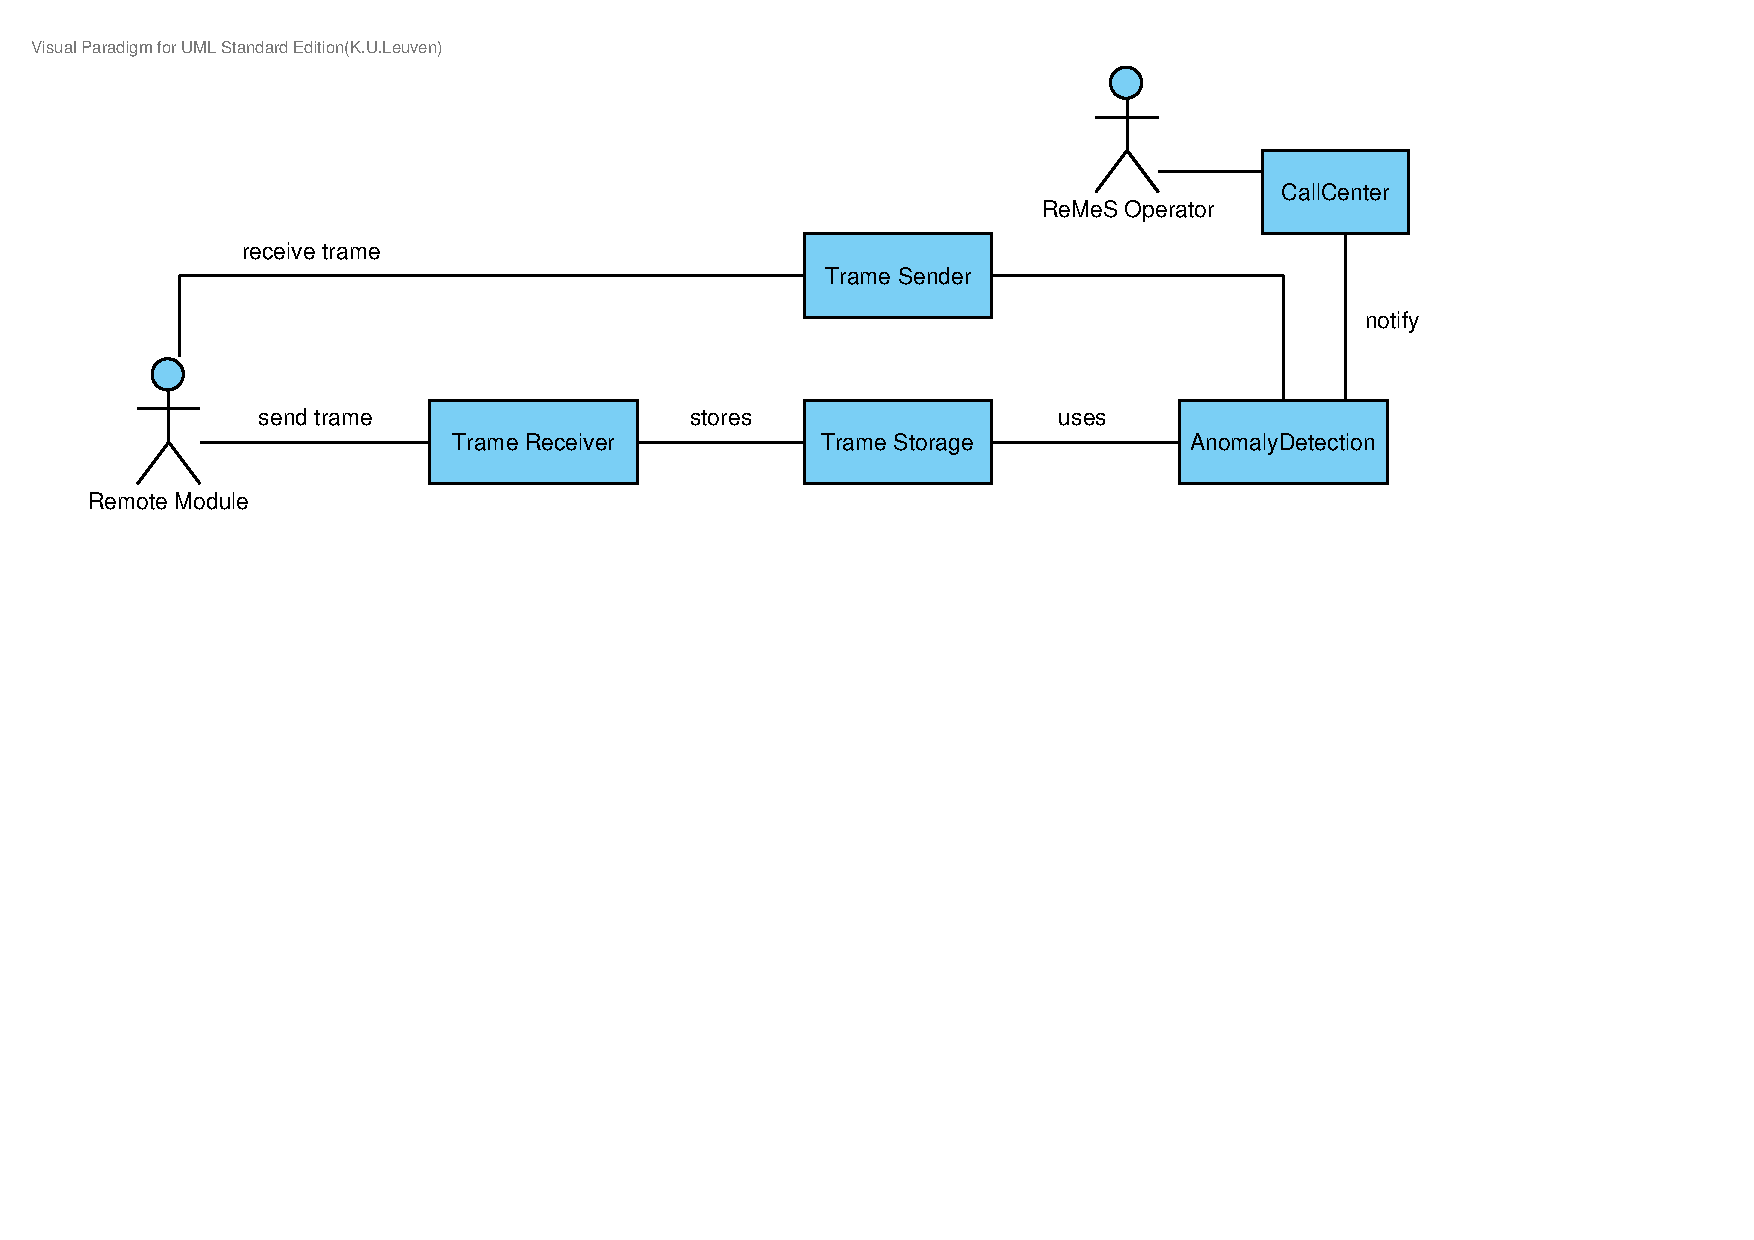
\includegraphics[width=0.6\textwidth]{figs/decomposition/whole-system/domainmodel-draft.pdf}
		\caption{Draft of the domain model used in the level 1 decomposition}
		\label{fig:dec/whole-system/draft}
	\end{centering}
\end{figure}

\subsubsection{Tactics}
\label{tactics:whole-system}



\subsubsection{Design Patterns}
\label{dp:whole-system}

\npar With respect to resource arbitration and resouce management, the
\emph{Active Object} design pattern is chosen for trame communication and
processing. Schedulers will determine the order in which trames are received,
processed and sent. These schedulers will have different scheduling policies,
implemented with the \emph{strategy} design pattern, in order to allow operation
in different modes.

\npar The trames will have to be objectified. This will yield two advantages.
Firstly, the scheduler can be implemented using the \emph{Command Processor}
design pattern. Secondly, a unified language will exist for all vendor
specific trame formats.

\npar To make the data highly available, the database will be replicated. This
can be achieved by using the \emph{Replicated Component Group} design pattern.
The database will be replaced with a front-end interface that replicates all
requests to all the replicas. 

\subsubsection{Other requirements}
\label{others:whole-system}


